\documentclass[pdflatex,compress,mathserif]{beamer}

%\usetheme[dark,framenumber,totalframenumber]{ElektroITK}
\usetheme[darktitle,framenumber,totalframenumber]{ElektroITK}

\usepackage[utf8]{inputenc}
\usepackage[T1]{fontenc}
\usepackage{lmodern}
\usepackage[bahasai]{babel}
\usepackage{amsmath}
\usepackage{amsfonts}
\usepackage{amssymb}
\usepackage{graphicx}
\usepackage{multicol}
\usepackage{lipsum}
\usefonttheme[onlymath]{serif}

\newcommand*{\Scale}[2][4]{\scalebox{#1}{$#2$}}%

\setbeamertemplate{caption}[numbered]

\title{PENGOLAHAN SINYAL DIGITAL}
\subtitle{Pengantar Pengolahan Sinyal Digital}

\author{Mifta Nur Farid}

\begin{document}

\maketitle

\section{Konsep Dasar Pengolahan Sinyal Digital}

\begin{frame}{Skema Pengolahan Sinyal Digital}
	\begin{figure}
		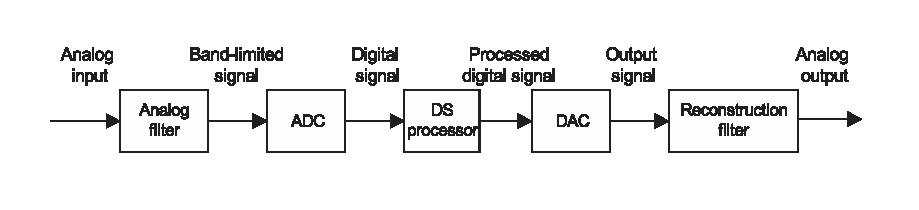
\includegraphics[width=\linewidth]{img/img01}
	\end{figure}
\end{frame}

\section{Contoh Dasar Pengolahan Sinyal Digital dalam Diagram Blok}

\subsection{Filter Digital}

\begin{frame}{Blok Filter Digital Sederhana}
	\begin{figure}
		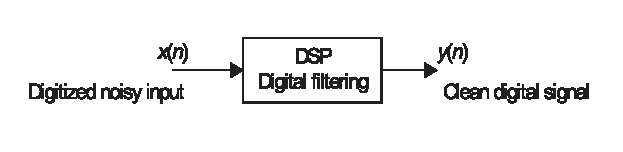
\includegraphics[width=\linewidth]{img/img02}
	\end{figure}
\end{frame}

\begin{frame}{Blok Filter Digital Sederhana}
	\begin{figure}
		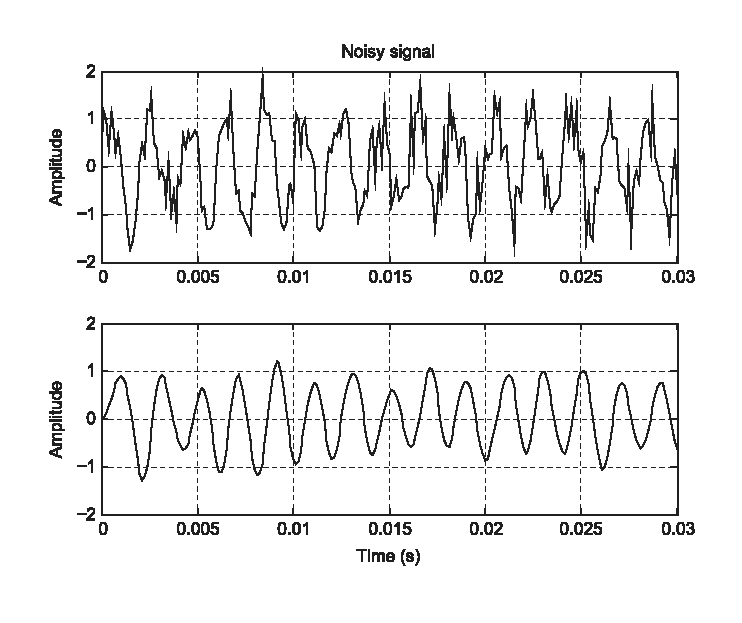
\includegraphics[width=0.8\linewidth]{img/img03}
	\end{figure}
\end{frame}

\subsection{Analisis Frekuensi Sinyal (Spektrum)}

\begin{frame}{Sinyal Audio dan Spektrumnya}
	\begin{figure}
		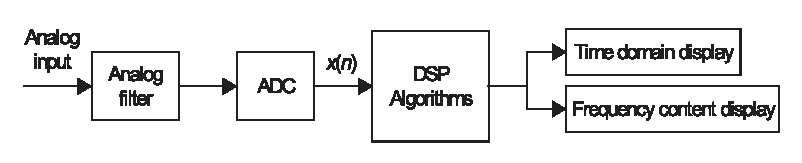
\includegraphics[width=\linewidth]{img/img04}
	\end{figure}
\end{frame}

\begin{frame}{Sinyal Audio dan Spektrumnya}
	\begin{figure}
		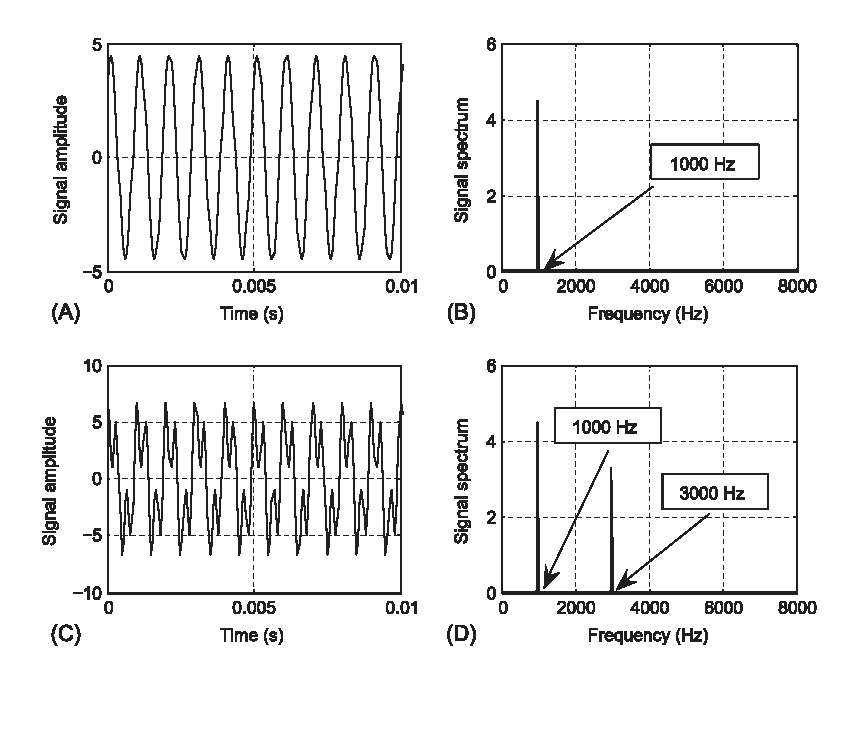
\includegraphics[width=0.8\linewidth]{img/img05}
	\end{figure}
\end{frame}

\begin{frame}{Sinyal Suara dan Spektrum Suara}
	\begin{figure}
		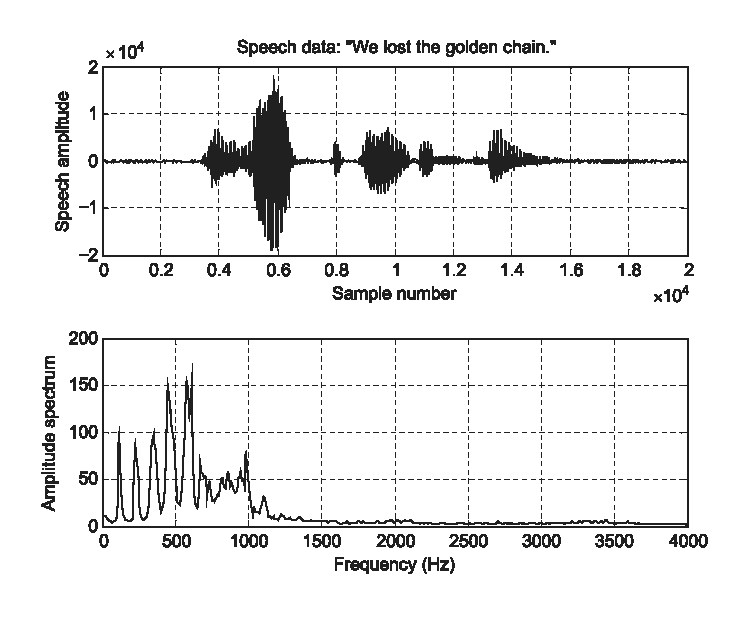
\includegraphics[width=0.8\linewidth]{img/img06}
	\end{figure}
\end{frame}

\section{Gambaran Pengolahan Sinyal Digital dalam Penerapannya di Dunia Nyata }

\subsection{Sistem Audio Crossover Digital}

\begin{frame}{Two-band digital crossover}
	\begin{figure}
		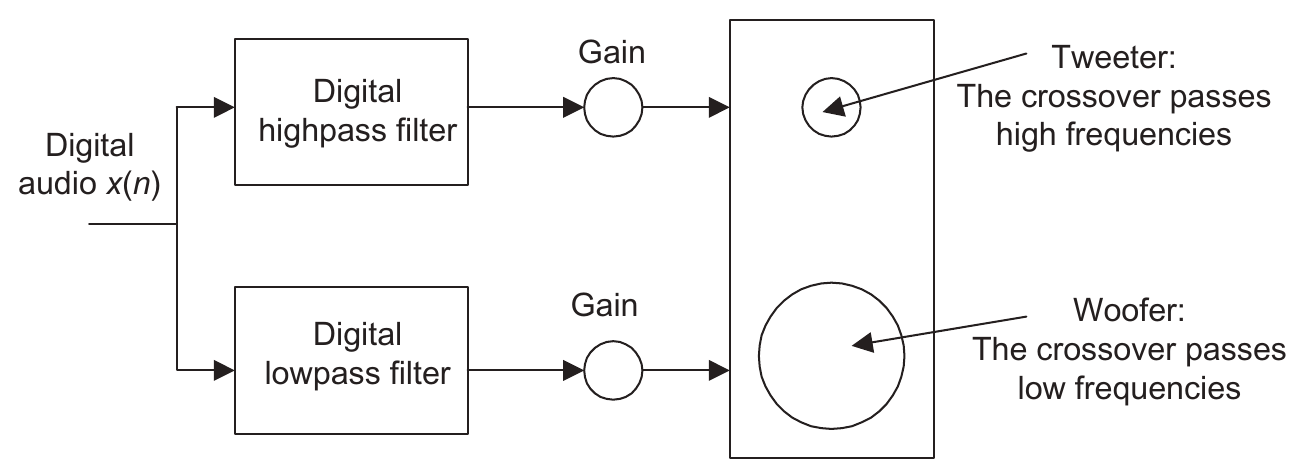
\includegraphics[width=0.8\linewidth]{img/img07}
	\end{figure}
\end{frame}

\begin{frame}{Elimination of 60-Hz interference in electrocardiography (ECG)}
	\begin{figure}
		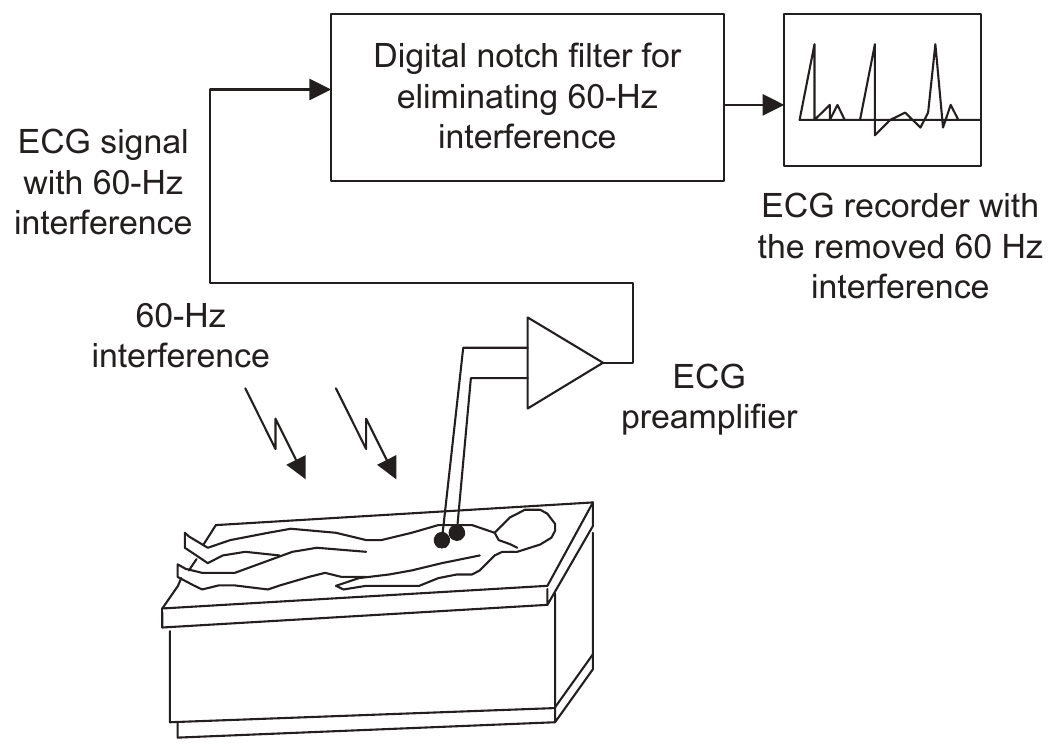
\includegraphics[width=0.8\linewidth]{img/img08}
	\end{figure}
\end{frame}

\begin{frame}{Simplified data compressor and Simplified data expander (decompressor)}
	\begin{figure}
		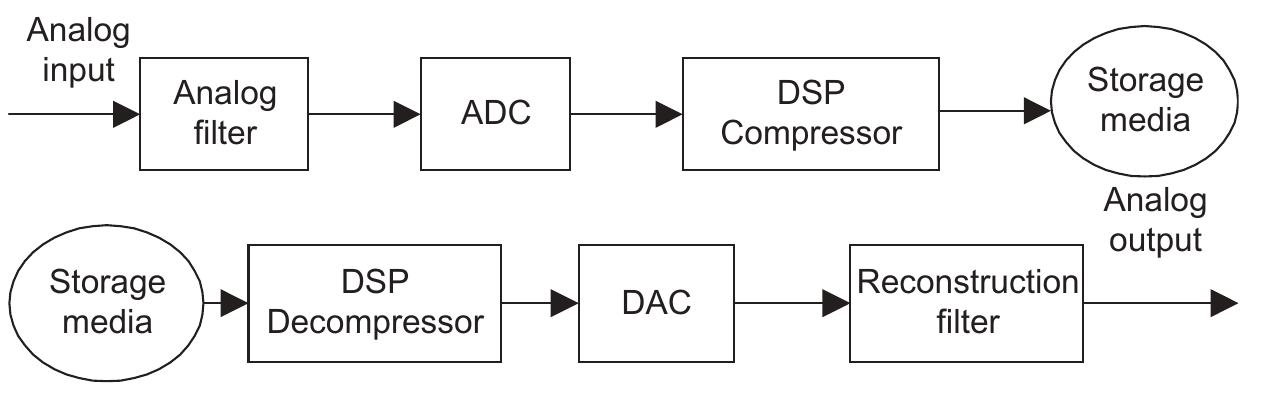
\includegraphics[width=0.8\linewidth]{img/img09}
	\end{figure}
\end{frame}

\begin{frame}{Simplified encoder of the CD recording system and Simplified decoder of the CD recording system}
	\begin{figure}
		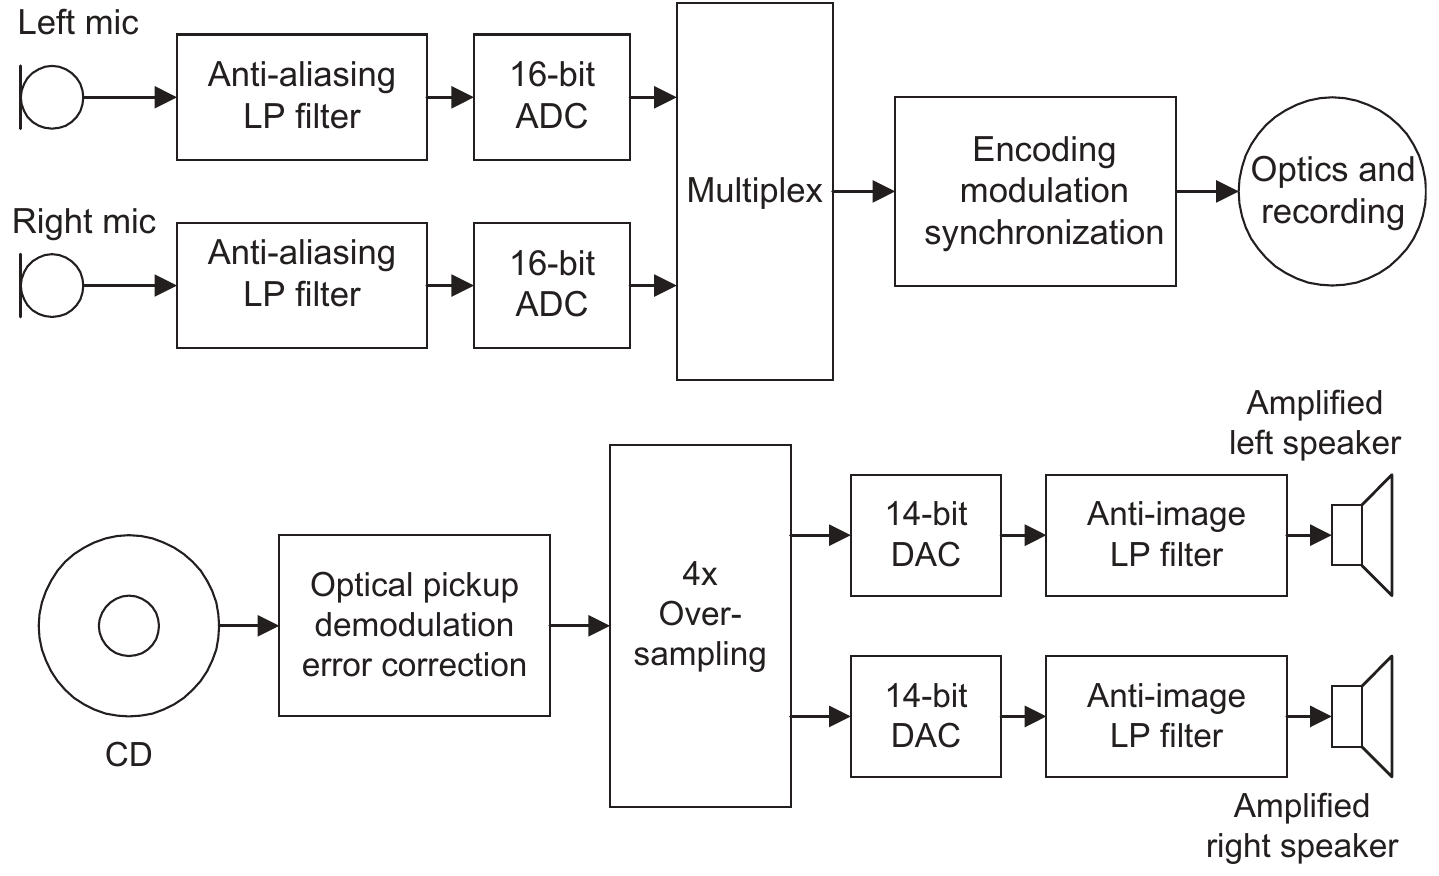
\includegraphics[width=0.8\linewidth]{img/img10}
	\end{figure}
\end{frame}

\begin{frame}{Vibration signature analysis of the gearbox}
	\begin{figure}
		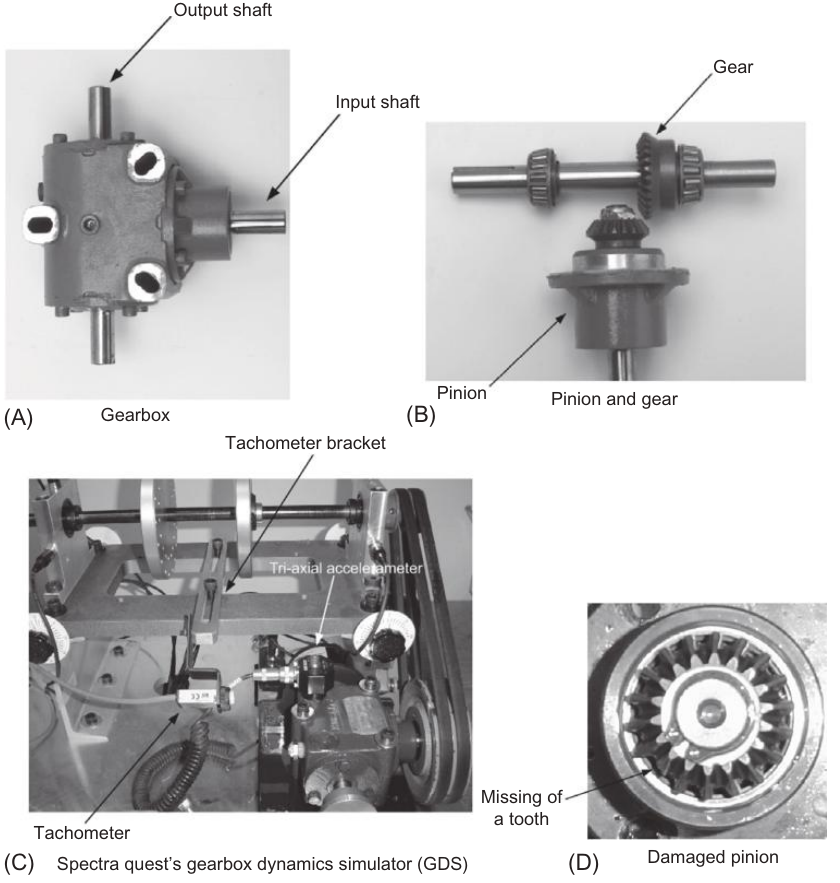
\includegraphics[width=0.5\linewidth]{img/img11}
	\end{figure}
\end{frame}

\begin{frame}{Vibration signal and spectrum from the good condition gearbox}
	\begin{figure}
		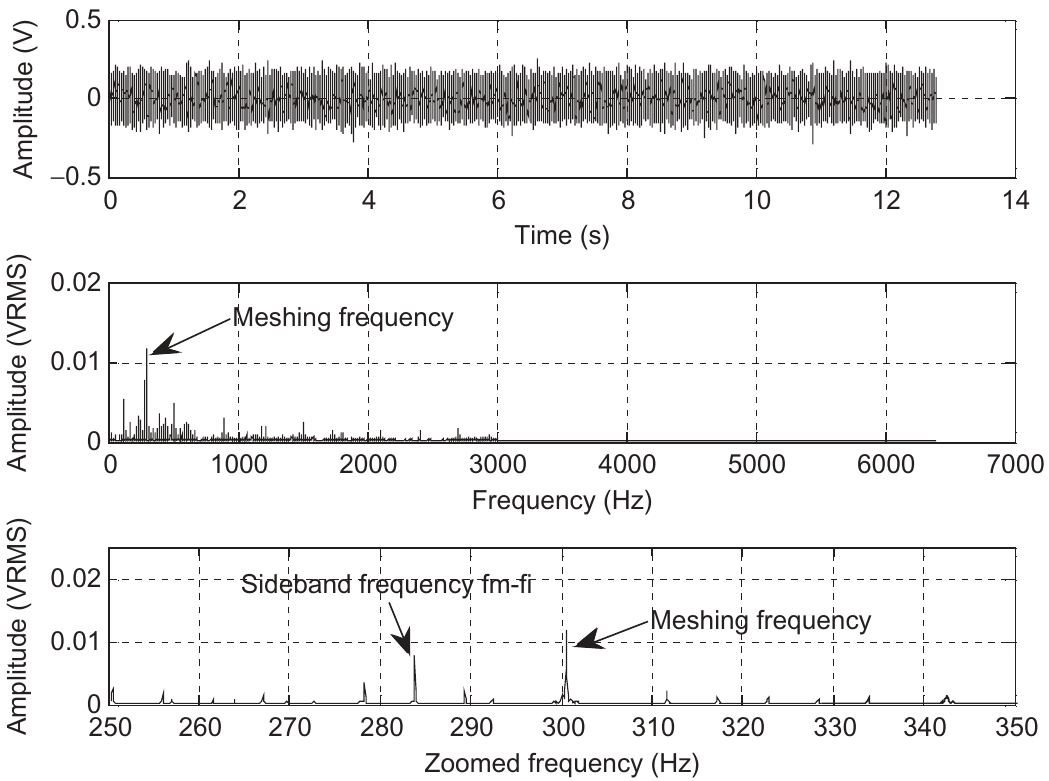
\includegraphics[width=0.8\linewidth]{img/img12}
	\end{figure}
\end{frame}

\begin{frame}{Vibration signal and spectrum from the damaged gearbox}
	\begin{figure}
		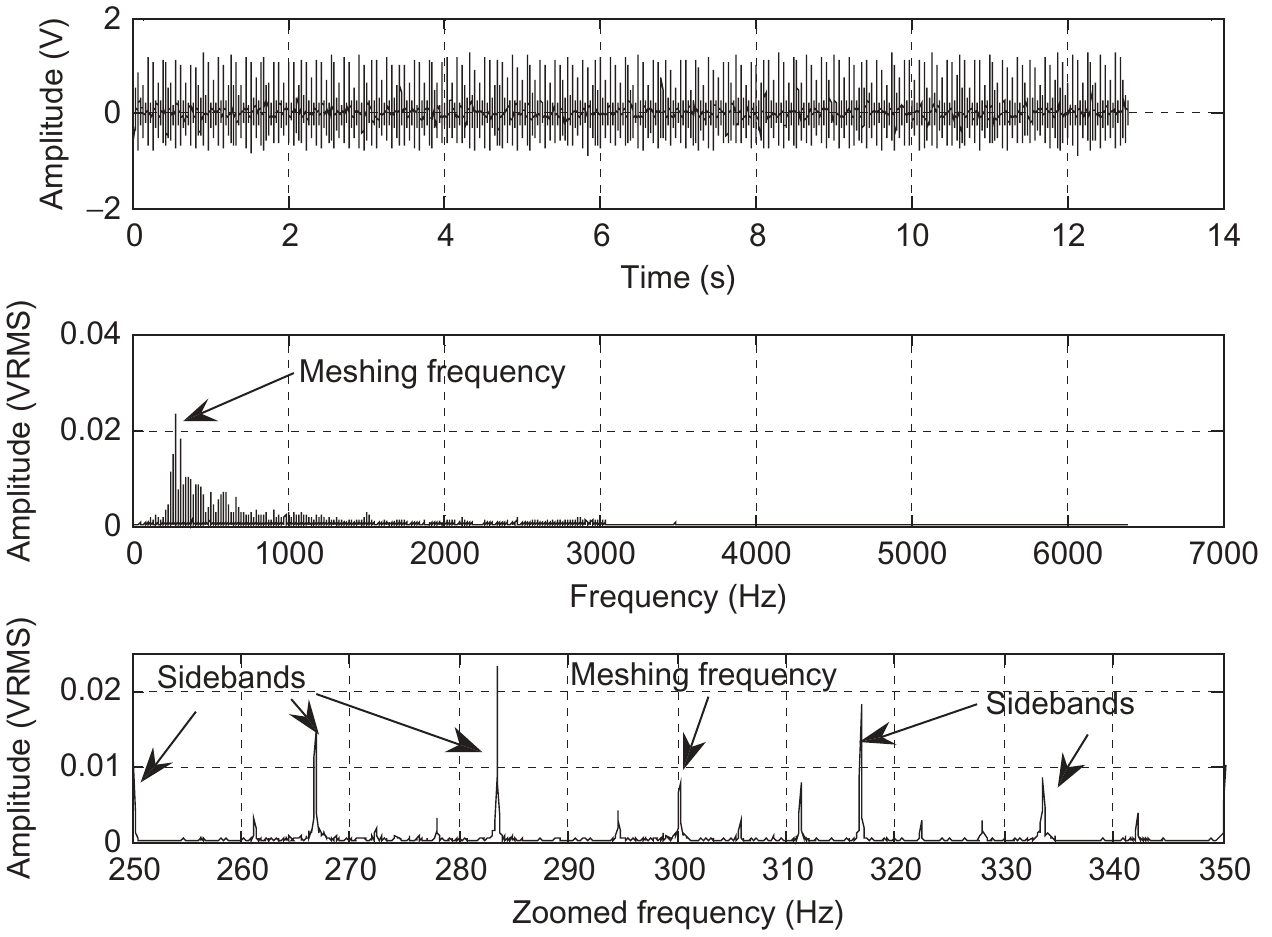
\includegraphics[width=0.8\linewidth]{img/img13}
	\end{figure}
\end{frame}

\begin{frame}{Image enhancement.}
	\begin{figure}
		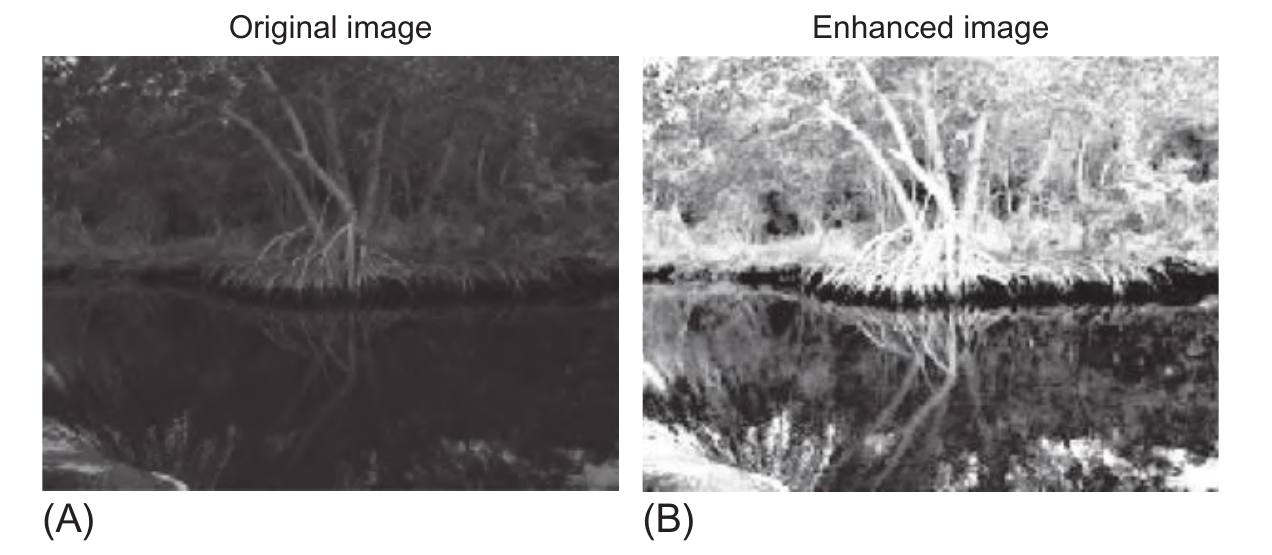
\includegraphics[width=\linewidth]{img/img14}
	\end{figure}
\end{frame}

\begin{frame}{Applications of Digital Signal Processing}
	\begin{figure}
		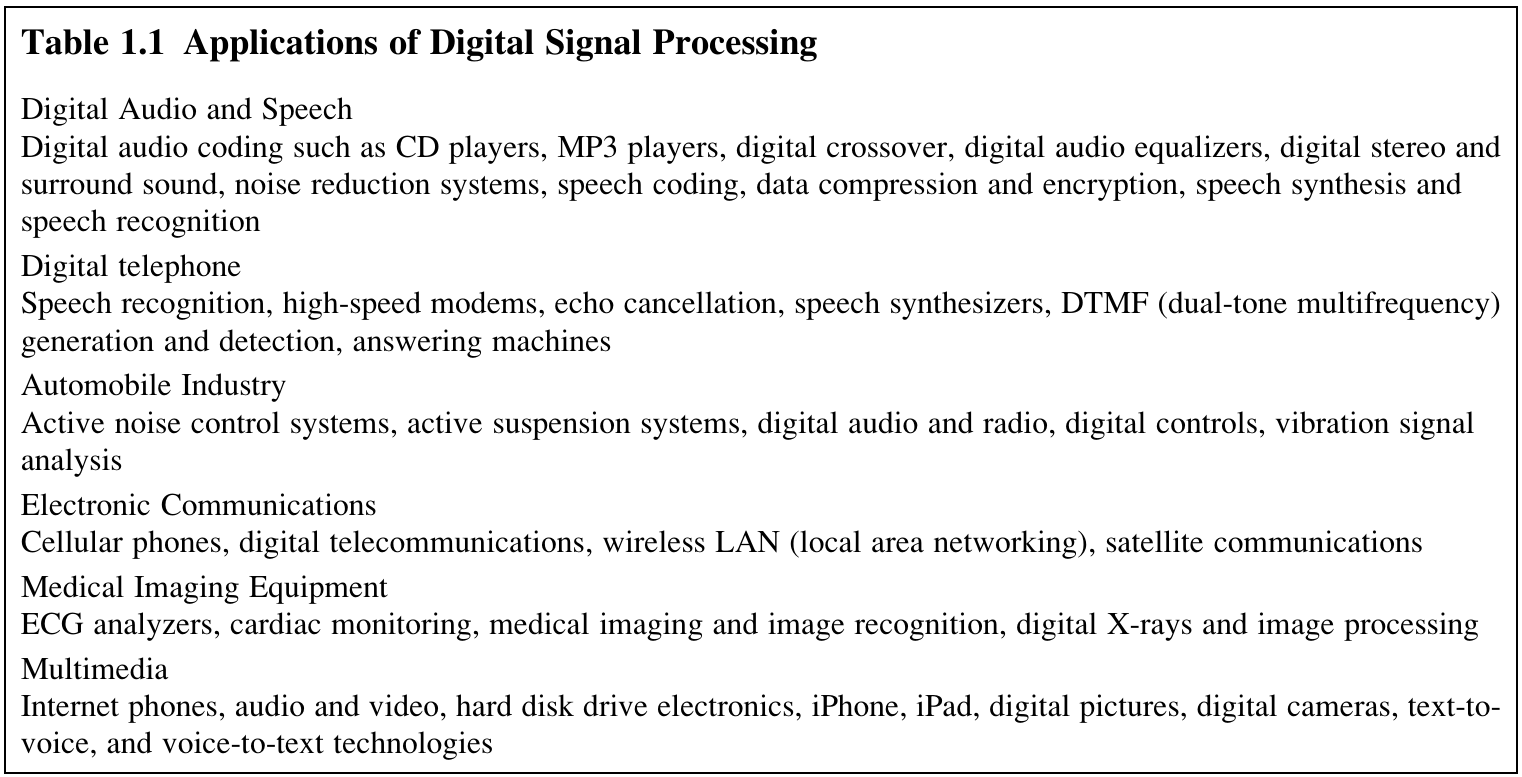
\includegraphics[width=\linewidth]{img/img15}
	\end{figure}
\end{frame}

\end{document}
